% !TEX root = ../rawlik-phd-thesis.tex
\chapter{Axion analysis}
\label{ch:axion-analysis}

Now that the foundation of the analysis has been introduced, we describe how it was applied to look for oscillations in the neutron EDM data taken at the PSI in the years 2015--17.

First we considered the scalar coupling, acting like an oscillating nEDM signal. We analysed directly the time series of $R$, measured with every cycle of the experiment. This allowed us to consider frequencies up to inverse \SI{300}{\second}, but, on the other hand, required a careful consideration of the effect that on oscillating nEDM would would have on the $R$ time series. Not having found a signal, we could interpret this analysis as the first laboratory limits on the axion coupling to gluons.

The work described in this chapter was a joint effort with Nicholas Ayres, who analysed the data of the Grenoble-based nEDM measurement~\cite{AyresThesis} in search for the scalar coupling. Rather than the raw $R$ time series, he considered the one of the nEDM estimates as obtained on a run basis. The two analyses were complimentary, each covering a different range of oscillation frequencies.

Then we discuss a different coupling, a vector one, acting like on oscillating magnetic field. No significant discovery could be claimed here, which led to exclusions for the axion-nucleon coupling.

Finally, we considered a particular frequency of \num{23.934}~hours, the sidereal frequency.
\marginpar{The sidereal frequency is the one of the Earth spinning in the celestial coordinates.}
Oscillations of that periodicity can be interpreted a hint of a \emph{cosmic spin anisotropy field}~\cite{Altarev2009}.



\section{How a signal would look like}
We start by considering, how an oscillating electric dipole moment would have come up in the $R$ time series, as measured by the PSI experiment.

The main purpose of the experiment was to measure the static neutron electric dipole moment. This would appear as a shift in $R$ dependent on direction of the electric field relative to the magnetic one. In a zero electric field there would be no shift, while the parallel and anti-parallel configurations of the magnetic and electric fields would shift $R$ in opposite directions. Due to the data blinding
% \footnote{In order to reduce bias the data were modified upon being taken in a way, that a secret nEDM was injected into them. This additional offset is only revealed as the very last step, once the measurement and analysis have been completed. The data were still blinded at the time of writing.}
we expect a pronounce shift corresponding to an nEDM of \SI{e-25}{\elementarycharge\centi\meter}.

Should the neutron electric dipole moment oscillate, $R$ would oscillate as well, even if the electric field is kept constant. A reversal of the electric field polarity would reverse the phase of the oscillations. At zero electric field no oscillations would be visible. In the PSI experiment the field was automatically changed according to the looped pattern: 48 cycles in one polarity, 8 cycles without the field, 48 cycles in the other, 8 without the field. In Fig.\,\ref{fig:axions_data_taking_one_run} we depict an $R$ time series with the combined effect of a large nEDM oscillation and the blinding offset.

\begin{figure}
  \centering
  \subfloat[An oscillating neutron electric dipole moment signal in the nEDM @ PSI apparatus. The colours indicate different electric field states: parallel to the magnetic field, antiparallel to it and zero]
  {\label{fig:axions_data_taking_one_run}
  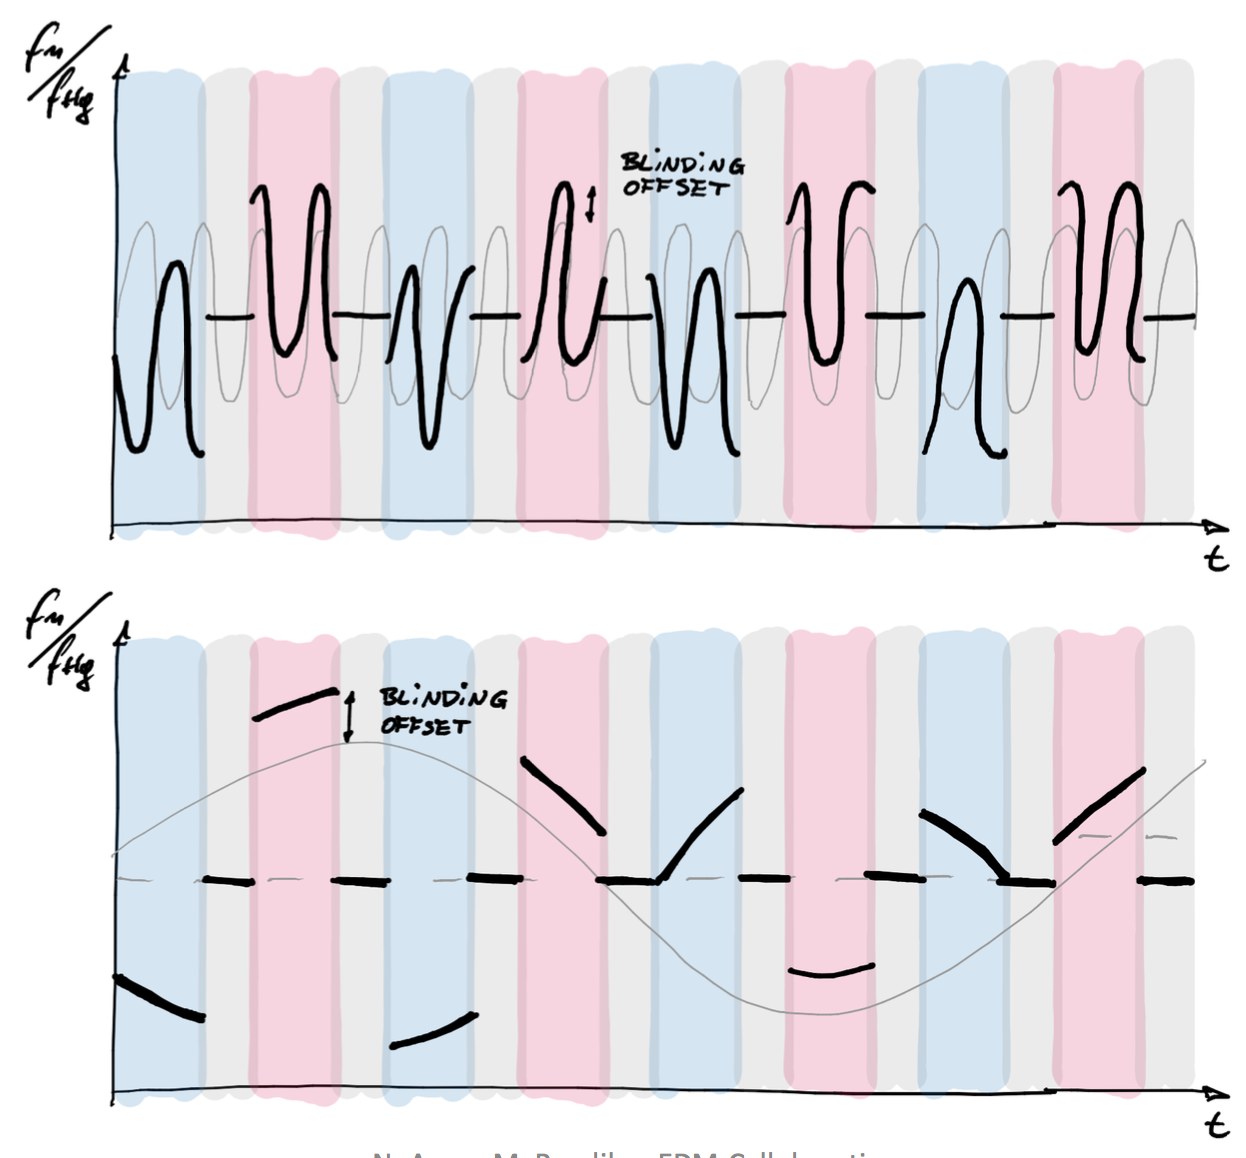
\includegraphics[width=.34\linewidth]{gfx/axions/cycle-level_blinding_offset.png}}
  \quad
  \subfloat[An oscillating neutron electric dipole moment signal in the nEDM @ PSI apparatus across many runs. The colours indicate different electric field states: parallel to the magnetic field, antiparallel to it and zero. Different runs have different magnetic field gradients, which causes each run to have a different shift in $R = f_n / f_{Hg}$.]
  {\label{fig:axions_data_taking_runs}
  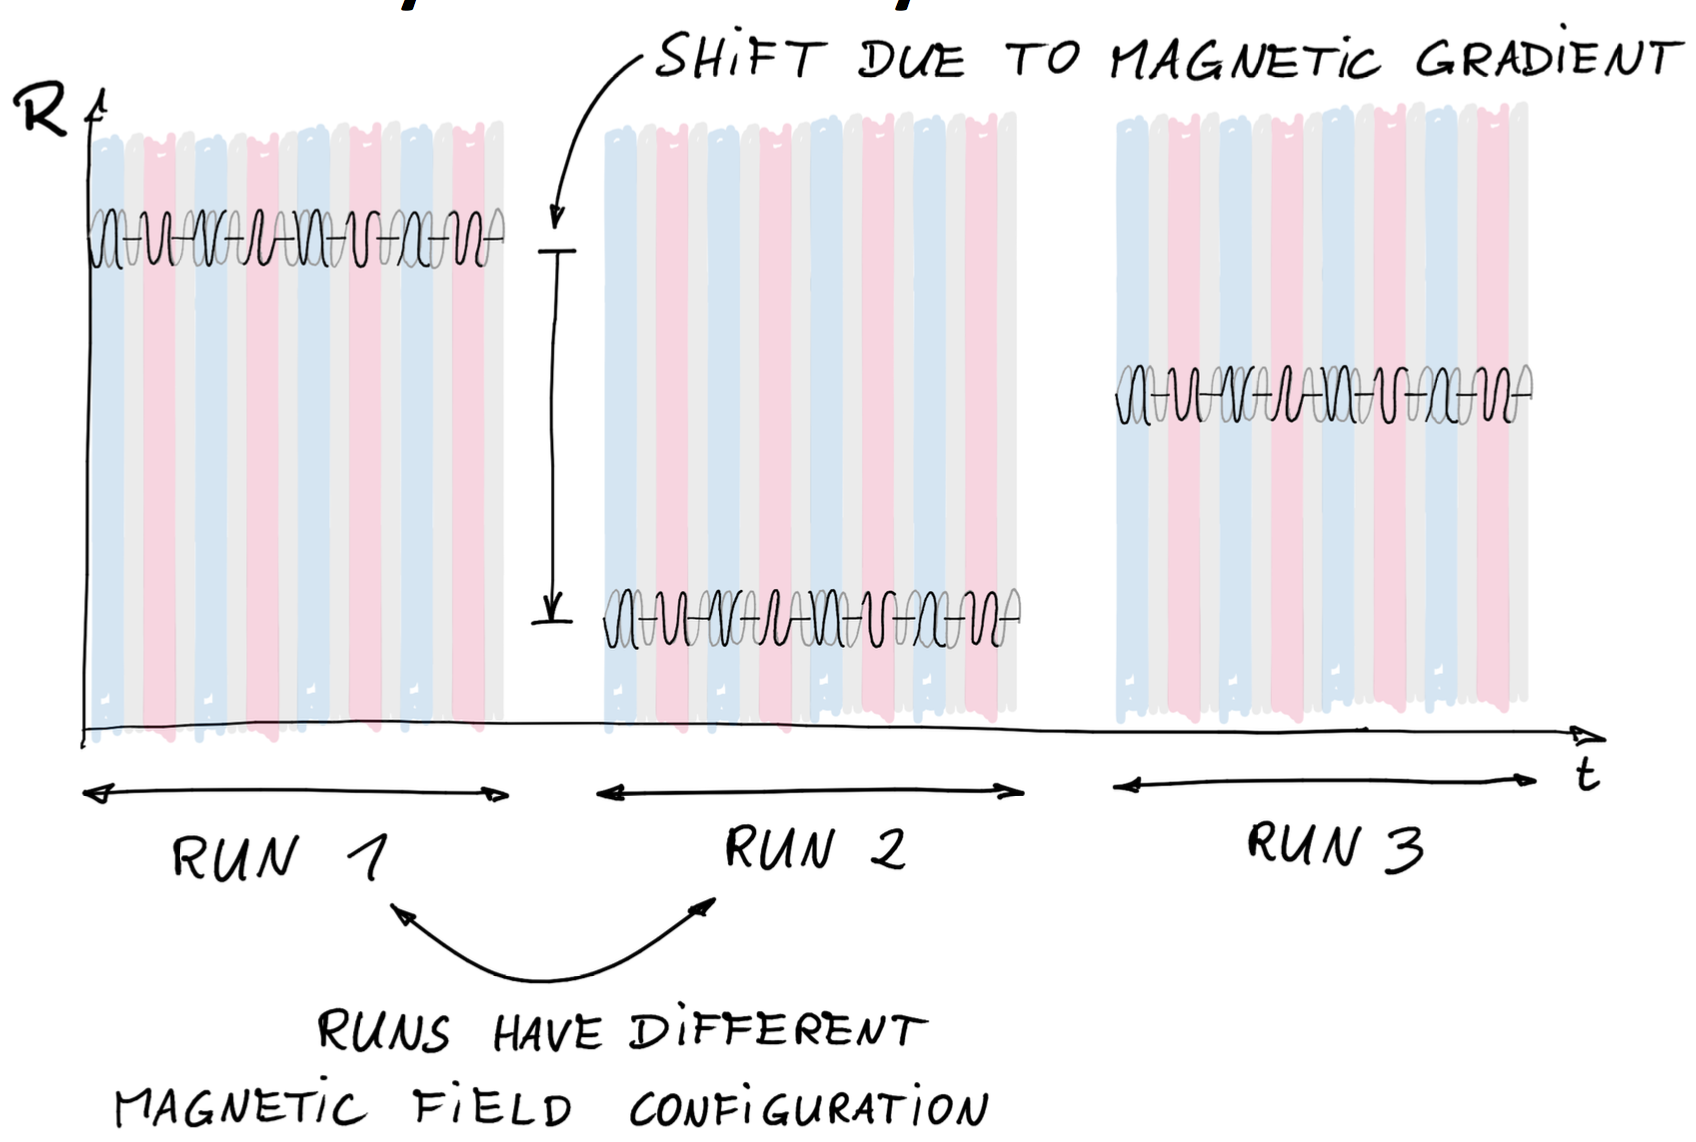
\includegraphics[width=.56\linewidth]{gfx/axions/cycle-level_gradient_jump.png}}
  \caption{The data taking scheme in the nEDM experiment at PSI.}
\end{figure}

Of course, the least-squares spectral analysis could not be applied directly to the complicated $R$ time series. Note, that the time series is still a part of a harmonic oscillation, when only one electric field polarity is considered. Or, to be exact, one relative configuration of the electric and magnetic fields. In the analysis the $R$ time series was split according to this condition into three: one without the electric field (not sensitive to an oscillation of nEDM), one with the electric and magnetic fields parallel and one with anti-parallel. The last having the hypothetical oscillation in the opposite phase then the parallel one. We will refer to the three data sets as $E=0$, $E \uparrow \uparrow B$ and $E \uparrow \downarrow B$, respectively. Each of those was treated separately.

% \begin{figure}[bth]
%   %FIXME directly copied from Elise's presentation on the 2015 PSI collaboration meeting
%   \myfloatalign
%   \subfloat
%   [Another time series of $R$ in the nEDM experiment. The colours depict electric field states, black being no electric field. A drift is clearly visible.]
%   {\label{fig:axions_gradient_drift_not_corrected}
%   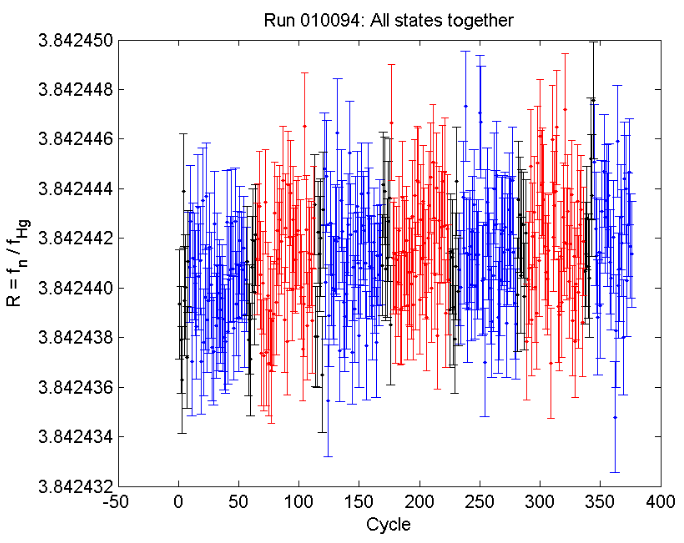
\includegraphics[width=.45\linewidth]{gfx/axions/gradient_drift_elise}}
%   \quad
%   \subfloat
%   [The data as on Fig.\,\ref{fig:axions_gradient_drift_not_corrected} corrected for gradient fluctuations.]
%   {\label{fig:axions_gradient_drift_corrected}
%   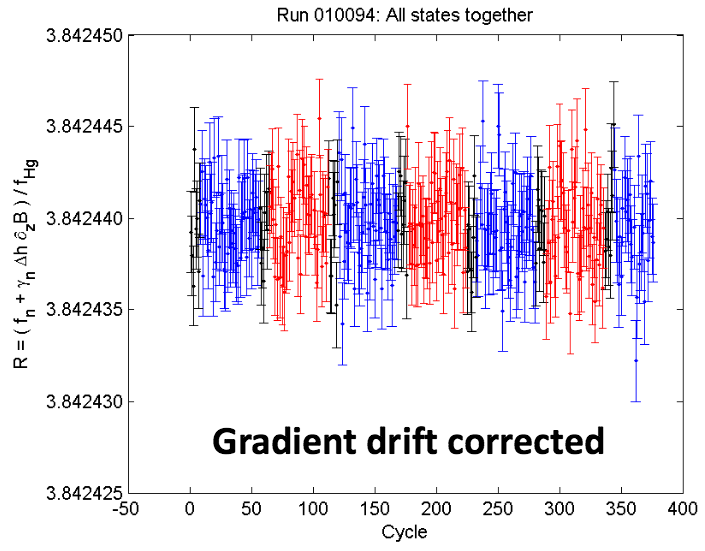
\includegraphics[width=.45\linewidth]{gfx/axions/gradient_drift_elise_corrected}}
%   \caption{Correcting the $R$ time series for fluctuations of the vertical magnetic field gradient.}
%   \label{fig:axions_gradient_drift_correction}
% \end{figure}

There are other effects in the $R$ time series. A part of the measurement procedure was to deliberately work in a magnetic field gradient, as discussed in Sec.\,\ref{sec:measurement_procedure}. The vertical magnetic field gradient changed substantially between sequences. Thereby $R$ was affected by a big value, changing the DC level of the oscillating nEDM signal, as illustrated in Fig.\,\ref{fig:axions_data_taking_runs}.

The problem of inter-sequence jumps was solved by allowing the DC offset in the LSSA fit to be different in each sequence:
\begin{equation}
  \label{eq:axions_LSSA}
  A\sin(2 \pi f t) + B\cos(2 \pi f t) + \sum_i C_i\,\Pi_i(t) \ ,
\end{equation}
where $C_i$ is the free offset in the $i$th sequence and $\Pi_i(t)$ is a gate function equal to one in the $i$th sequence and zero elsewhere. In this way the model explicitly assumed coherence of the oscillation across sequences. However, the downside was a reduced sensitivity to oscillations slower than a sequence (2--3 days), as they could be absorbed into the different free offsets. This, together with the split into three series, reduced the problem to one described in the previous chapter.

% It may be tempting to think about demodulating the $R$ time-series into what would be expected to be an oscillation. This would require subtracting the DC offset for each electric field configuration, in each run separately, then flipping the signal around the DC level for one configuration. \mnote{The offsets are measured with Cs, mention that.} The disadvantage is that uncertainty in such a demodulation would become a systematic effect and would need to be tightly controlled.

% , as clearly visible in Fig.\,\ref{fig:axions_gradient_drift_correction}.
% The nEDM team spares no effort to measure the gradient. Nevertheless, the achieved precision (\SI[per-mode=symbol]{\approx 1}{\pico\tesla\per\centi\meter}) is only comparable to the one of $f_n$ (in the order of \SI{1}{\pico\tesla}). The exact way how the gradient should determined is highly non--trivial and there is ongoing research in this respect. \mnote{Mention here the exact way the gradient drift correction is done. And cite Elise's thesis.} Actually, even the height difference between the neturons and $^{199}$Hg centres of mass (a few milimeters) is still discussed. \mnote{Know how exactly was $\Delta h$ determined in the end. Also, mention the definition of a sequence here (as in the paper).}
% \cite{Afach2014magmoment}

% Assuming a constant gradient during a \emph{run} one can determine it much more precise. This assumption, however, is known not to be exactly true.

% One should note, that any, including an oscillating one, nEDM effect affects only the position of the neutrons' resonance. The shape of the resonance curve is unaffected. Therefore, the method to extract neutron Larmor frequency $f_n$, and thereby $R$, for each \emph{cycle} is valid also in case of an oscillating nEDM.



\section{Systematic Effects}
In the analysis the compatibility of the periodogram of the $R$ time series with the one of pure noise, the null hypothesis, was tested. Variations in $R$, harmonic in particular, but not only, would have resulted in an additional power in the periodogram and could, therefore, be considered a systematic effect.

Most prominently, $R$ followed the changes in the vertical gradient of the magnetic field. Because of the centre of height difference between the neutron and mercury atom ensembles they saw, on average, a different field in a presence of the vertical gradient.  Luckily, it could be corrected for with the use of the cesium magnetometers. On a cycle basis, a second-order parametrisation of the field was fitted to their readouts, giving an estimate of the gradient~\cite{Afach2014magmoment,WurstenThesis}. Due to unknown random offsets in the magnetometers' readings the correction was only relative---correcting for the variations of the gradient. In between runs the caesium magnetometers were calibrated, which altered the offsets. For this reason the correction could not extend across a run boundary. 
% , which changed in between runs which changing after this correction could only be relative in a run.
% \marginpar{STILL CHANGE RUN TO SEQUENCE!!!}

There could have been, potentially, other effects causing the time series of $R$ not to be fully random. An important decision had to be taken on how to treat those. Two possibilities were considered.

A detail study of time-dependent systematic effect could be performed.
Here any excess in power, in any dataset ($E \uparrow \uparrow B$, $E \uparrow \downarrow B$ and $E=0$) would be treated as a signature of some kind of a signal. All effects that could potentially result in that would have to be identified before the analysis was performed and corrected for. This would have required a long and careful systematic study. Moreover, the full-fledged systematic studies for the constant nEDM analysis of the PSI data were still ongoing at the time. This approach was considered to be, albeit careful, not necessary for this analysis.

% \paragraph{Determine delicate frequencies and cut them out.}
% The experiment run 
% Looking at periodograms of raw data one sees that there are several typical frequencies where peaks appear. Typically at inverse specific time constants at which the experiment operates: cycle separation, day, week, , HV-reversal, B0-reversal. We may decide that all systematic effects are constrained to these frequencies and do not perform the analysis there at all.

% \paragraph{Assume there are no systematic effects.}
Instead, an easier approach was taken. An axion would produce a very specific signal, in particular:
\begin{enumerate}
  \item There would be no signal in the $E=0$ dataset.
  \item The signal would appear in both $E \uparrow \uparrow B$ and $E \uparrow \downarrow B$ datasets, with equal amplitude.
  \item The signals in $E \uparrow \uparrow B$ and $E \uparrow \downarrow B$ data sets would be shifted in phase by \ang{180}.
  \item The signals would have to have a high coherence of $\delta f / f = 10^{-6}$.
\end{enumerate}
In a case when an excess in the power would be observed, it would only be called a candidate for an axion signal, if the three above conditions would have been met. Otherwise, it would be attributed to a, potentially unknown, systematic effect.

Naturally, this made the systematic study dependent of the fact of having found a signal, opening a line of attack on the analysis. The analysis might be claimed not to have the right to exclude signals, because there might have been a systematic effect that cancelled a real signal out, but was never found nor even looked for. Nevertheless, such an event was highly improbable due to the high coherence of the axion field. In order to cancel the axion signal, a systematic effect would have not only needed to be as coherent as the axion field, but additionally fine-tuned over at least 5 orders of magnitude magnitude of tested frequencies. With the coherence of $\delta f / f = \num{e-6}$ this is a tuning of \num{e-30}. It would also have needed to be fine-tuned in amplitude over $\sim 20$ orders of magnitude, which gives a rough estimate of the cancellation probability of \num{e-50}. As the exclusions are anyway probabilistic in nature, in this case a 95\% C.L. threshold is claimed, we consider this approach to be justified.




\section{The PSI 2015--16 data set}
\note{uniform spelling of data set}

% What is it that I really want to communicate here? First introduce the time series and point to the plot. Then explain the structure by walking the reader through the plot!

\begin{figure}
  \centering
  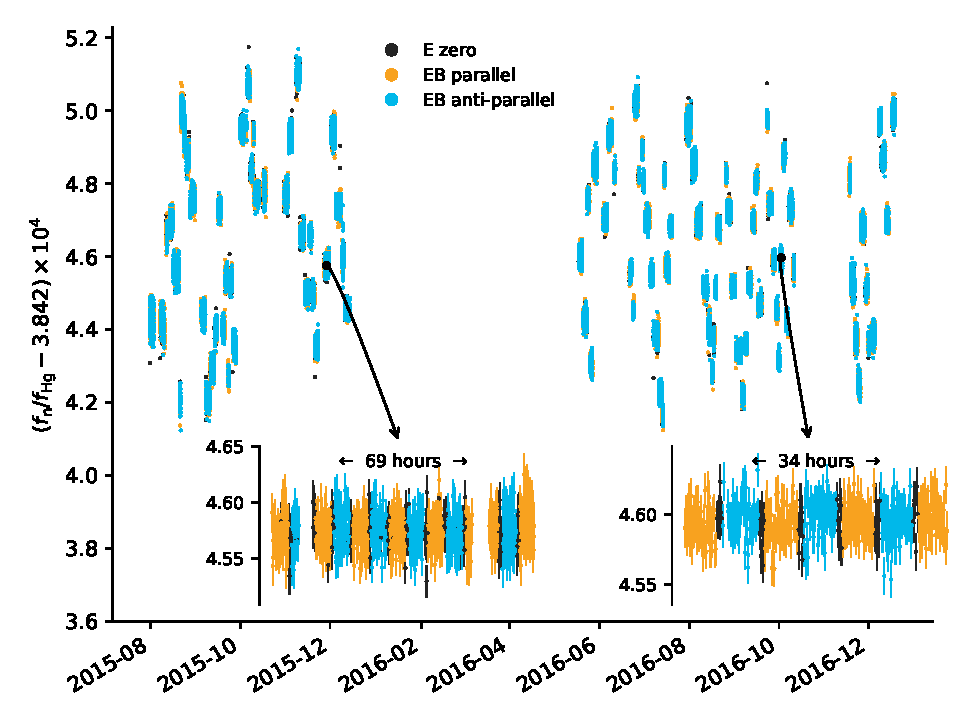
\includegraphics[width=0.9\linewidth]{gfx/axions/deltah4mm_time_domain_inset_no_yerr.pdf}
  \caption{The complete PSI data set used in the analysis. It spans from July 2015 to December 2016. Two sequences are enlarged. Due to high density of the measurements individual points cannot be resolved. Each point is plotted with its error bar. The colours depict the relative orientation of the magnetic and electric fields: $E \uparrow \uparrow B$ (orange), $E \uparrow \downarrow B$ (blue) and $E=0$ (black). The $R$ time series has been corrected for gradient drifts.}
  \label{fig:PSI_dataset_time_domain}
\end{figure}

The data used in the analysis were collected in PSI between 2015--07--03, 14:21:30 and 2016--12--18, 19:51:23. The measurements were performed primarily to obtain the estimate of the constant nEDM\@. The time series of the ratio of the precession frequencies of the neutrons and mercury atoms $R = \nu_\text{n} / \nu_\text{Hg}$ is presented in Fig.\,\ref{fig:PSI_dataset_time_domain}.

Take a look first at the inset in the lower-right corner. It zooms into data collected within one \emph{sequence}, typically 1--3 days long.
\marginpar{A technical term for uninterupted operation was a run. Sometimes a run was stopped due to technical reasons a new started afterwards. A sequence combines those consecutive runs, that could be one run if not for the interruption.}
During a sequence the apparatus completed one cycle after another, one every \SI{300}{\second}, each yielding an estimate of $R$.
The electric field was automatically changed between three states: pointing upwards, being zero and pointing downwards. The different relative orientations of the electric and magnetic fields are depicted in colour in the figure. Sometimes there were technical breaks in the data taking during a sequence, as in the case of the one shown in the lower-left corner of Fig.\,\ref{fig:PSI_dataset_time_domain}.

% Here what it is and what's done Sometimes the automatic process was interrupted, but the sequence still continued, as seen in the other inset.

% REFER TO WHAT WAS IN HOW THE SIGNAL WOULD LOOK LIKE! But, repeating a bit will not hurt. The reader should already be prepared, now just reiterate.

% \mnote{Idea: present a scheme of the timing structure of the nEDM data taking, where a cycle, sequence are defined, and HV and B field reversals are shown.}
% The time structure ias follows: The atomic measurement is called a cycle, which gives an estimate of the average precession frequency of the neutrons $f_\mathrm{n}$ and mercury $f_\mathrm{Hg}$. Their ratio $R = f_\mathrm{n} / f_\mathrm{Hg}$ is show in Fig.\,\ref{fig:PSI_dataset_time_domain}. An automatic system executes one cycle after another (triggered on a signal from the UCN source). A series of automatically executed cycles is called a \emph{run}. The $R$ time series of a typical run, 1-3 days long, is shown in the lower-right corner. During a run the electric field automatically changes polarity every \ldots \mnote{Find out how many cycles for one HV cycle} cycles. In between \ldots cycles with no electric field are measured. These have no sensitivity to the electric dipole moment, but provide a control data set.

A sequence was taken always in one magnetic field configuration. The in-sequence variations of the vertical gradient of the magnetic field $\partial_z B_z$ were corrected for using the field model fits to the readings of the Caesium magnetometers. In between the sequences the vertical gradient was changed in \SI{10}{\pico\tesla} steps, up to \SI{60}{\pico\tesla}, so that those systematic effects, which scale linearly with the gradient, could be extrapolated to zero (see Sec.\,\label{sec:measurement_procedure}). These large changes in the vertical gradient caused the large shifts in $R$ from sequence to sequence.

The $R$ time series was sliced into three separate based on the relative direction of the magnetic and electric fields: $E \uparrow \uparrow B$, $E \uparrow \downarrow B$ and $E=0$. In each a search for a harmonic oscillation was performed.

% During a single run the magnetic field is kept as stable as the team can manage. The drifts of the homogeneous part of the field are cancelled in $R$, but the gradients are not. So drifts of the gradient directly cause changes in $R$. These, however, can be corrected for using the Cs magnetometers. They are mounted on the top and bottom electrode and they can be used to correct for the in-run gradient drifts. They do not provide an accurate measure of the gradient. \mnote{Remember the reasoning why the cross-run gradient-drift correction can't be done: to large a change and the calibration issues}.

% Sometimes for technical reasons there is a pause in the measurements. Then the collected data may still belong to one run One such sequence is shown in the lower-right inset in Fig.\,\ref{fig:PSI_dataset_time_domain}.

% Typically... Sometimes stopped... Define a sequence



% Really, really first, show some example runs. 



\section{The analysis itself}

We start by presenting the results and then proceed to a more in-depth discussion.

\mnote{Definitely put in the plots for all three analyses (E0, EBp and EBap)! But only in the appendix!}

\mnote{This does not need to be explained really in detail! Most of the things were already explained earlier\ldots}

\mnote{The largest missing piece is the Cs gradient-drift correction. What should I do with it? The correction should be introduced by now!}

\begin{figure}
  \centering
  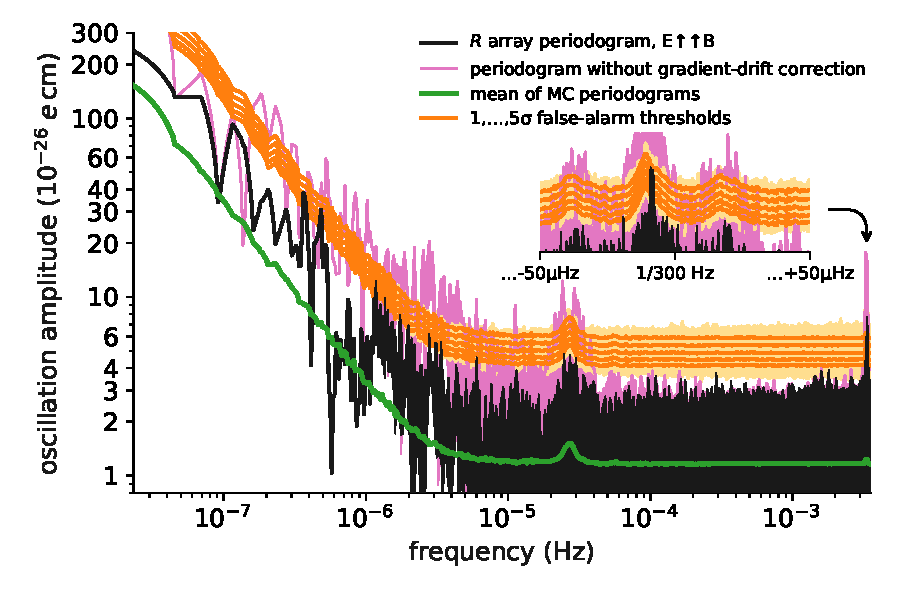
\includegraphics[width=0.9\linewidth]{gfx/axions/detection_psi_inset_gc.pdf}
  \caption{Periodogram of the $R$ time array of the PSI experiment data, sensitive to oscillations in the quantity $d_\mathrm{n} - \left( \mu_\mathrm{n} / \mu_\mathrm{Hg} \right) \, d_\mathrm{Hg}$, taken with the $\boldsymbol{E}$ and $\boldsymbol{B}$ fields parallel (black line).
  The mean of MC--generated periodograms, assuming no signal, is depicted in green. MC is used to calculate $1,2,…,5\,\sigma$ false--alarm thresholds, depicted in light orange.
  For clarity, we also plot the smoothed version in orange.
  There are two regions where a rise in the amplitude is expected, namely around \SI{28}{\micro\hertz} (inverse of 10 hours) and \SI{3.3}{\milli\hertz} (inverse of 300 seconds), due to the time structure of the data taking (see the main text for more details). The periodogram of non-gradient-drift-corrected data is shown in pink.}
  \label{fig:axions_PSI_detection}
\end{figure}

The periodogram of the subset of data with the electric and magnetic field parallel is presented in Fig.\,\ref{fig:axions_PSI_detection}.
There are two regions of expected rise in the oscillation amplitude due to the time structure of the data collection.
The one around $\unit[28]{\upmu Hz}$ (the inverse of 10 hours) corresponds to the period of the electric-field reversal.
The very narrow one around $\unit[3.3]{mHz}$ (the inverse of $\unit[300]{s}$) corresponds to the cycle repetition rate.
There are five
%\note{NA does anybody know what style guide says about when numbers should be written in words i.e. seven vs 7? I personally think small numbers without units should be words but this comes down to preference} ***I THINK LESS THAN TEN IT IS IN WORDS - MALCOLM ***
trial frequencies for which the $3\sigma$ false--alarm threshold is exceeded,
%\note{PMM: use words like 'surpassed', or 'exceeded' instead of penetrated}
two of which, including the largest excess with a $6\sigma$ significance, occur in a $\unit[100]{\upmu Hz}$ region around the inverse of \unit[300]{s}, while the other three are in the low-frequency region (inverse days) already excluded by the long time--base analysis.
% \note{FP: Can you maybe also explicitly state the positions of these three lines in Hz or inverse time?}
 The periodograms for the other two datasets (presented in \ref{ch:alp_appendix}) are very similar.
In the other sensitive set, there are three excesses of the $3\sigma$ threshold (the highest is $5\sigma$), all constrained to the same two regions. In the control dataset, only the $1\sigma$ threshold is exceeded.
%\note{MR: We may consider not discussing the false--alarm threshold penetrations, and just state in the next paragraph that we do not find a signal which meets our criteria.}
The periodogram of the $R$ time array without the gradient-drift correction is shown in pink in Fig.\,\ref{fig:axions_PSI_detection} to visualize the frequencies where the correction has an effect.

\mnote{Here a brief discussion about the Cs-gradient-drift correction.}
It is interesting to observe, that the periodograms with and without the gradient drift correction diverge only for frequencies below \SI{6e-5}{\hertz}, the period of the high-voltage reversal (the disagreement around inverse \SI{300}{\second} is folded from the low frequencies). This is not a coincidence. The period of the high-voltage reversal has been deliberately chosen, so that\ldots\mnote{Was the period really chosen such?}

No signals fulfilling the detection criteria are found.

Having observed no significant signal, we could place limits on the coupling strength as the function of axion mass.
The result are presented in Fig.\,\ref{fig:axions_limits_coupling} and are labeled \emph{short time-base} (the next paragraph is devoted to the \emph{long time-base} limits).
The limits we evaluated using Monte Carlo techniques, as described \ldots.
The results are presented in the landscape of already existing limits: axions with a mass below \ldots have their Compton wavelength larger than the size of the smallest dwarf \emph{galaxies} and, therefore, could not be the sole constituent of dark matter; the influence of axions in the red-shaded area on the \emph{Big Bang nucleosynthesis} would result in an underproduction of\ldots
\mnote{Need to research and explain all those.}

\begin{figure}
  \centering
  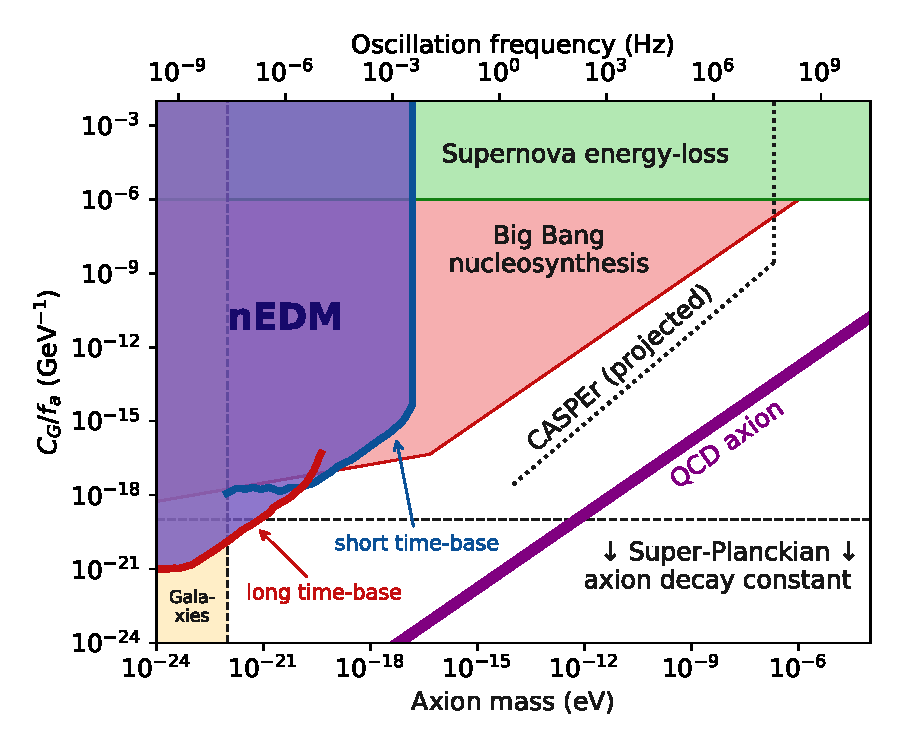
\includegraphics[width=0.9\linewidth]{gfx/axions/psi_ill_axion_limits_v7.pdf}
  \caption{Mention, that it shows\ldots}
  \label{fig:axions_limits_coupling}
\end{figure}

The Fig.\,\ref{fig:axions_limits_coupling} features the \emph{short time-base} limits, the ones described in this work, as well as \emph{long time-base} ones.
This work was performed with close collaboration with Nicholas Ayres of the University of Sussex. The Sussex group was part of the collaboration running the predecesor of the nEDM experiment at PSI --- the measurement performed in the Institute Laue-Langevin in Grenoble, France, in the years 1998--2002~\cite{Pendlebury2015}.
An analysis analogous to this work was performed on those data, with an important difference, which made it sensitive to lower frequencies (or lighter axions)~\cite{AyresThesis}.
Namely, the time series consisted of one point per run, in contrast to one per cycle in the short time-base analysis.
On one hand it limits the sensitivity to oscillation periods corresponding to one run (1--2 days).
On the other, the sensitivity to low frequencies is not deteriorated, as there is no need to use multiple free offsets in the LSSA fit (Eq.\,(\ref{eq:axions_LSSA})). In fact the free offset is assumed to be zero on the ground that the experiment delivered a zero-compatible result.
% in the process of calculating the per-run nEDM estimate the gradient fluctuations are averaged out, so there is 
\mnote{What about the gradient-related systematics (nEDM vs R' curve)? Was it corrected for? Wrote an email to Nick.}

Despite close collaboration the two analyses shared no common code. As a mean of cross-check, the two codes were compared on artifical datasets, more on that in the appendix.




\section{False-alarm thresholds}
\mnote{In this section we will dive in more deeply into statistics associated with the data.}

Remind: for each of the three data sets we have a periodogram, one value for the power estimate for each frequency. Then we have a collection of simulated periodograms, many power estimates for each frequency, generated assuming the null hypothesis --- only white noise in the data.

First how the local p-values were obtained. In Fig.\,\ref{fig:P_best_signal_candidate} the cumulative distribution function (CDF) \mnote{define CDF somewhere and then just continue to use it. Maybe even a table of abbreviations at the end?} of the power at one frequency (a special one, where the least probable peak is). CDF has this advantage over the PDF, that it does not require binning to be estimated. To estimate the CDF all the MC-generated power estimates are sorted into an array. Then the discrete CDF estimate is plotted by putting the power on the x-axis and the place in the sorted array, normalised to one, on the y-axis. Fig.\,\ref{fig:P_best_signal_candidate} actually shows $1 - \mathrm{CDF}$, so that the logarithmic y-scale can be leveraged to resolve the high-power tail. The plot also includes a extrapolating fit line and false--alarm thresholds, which we now proceed to explain.

\begin{figure}
  \centering
  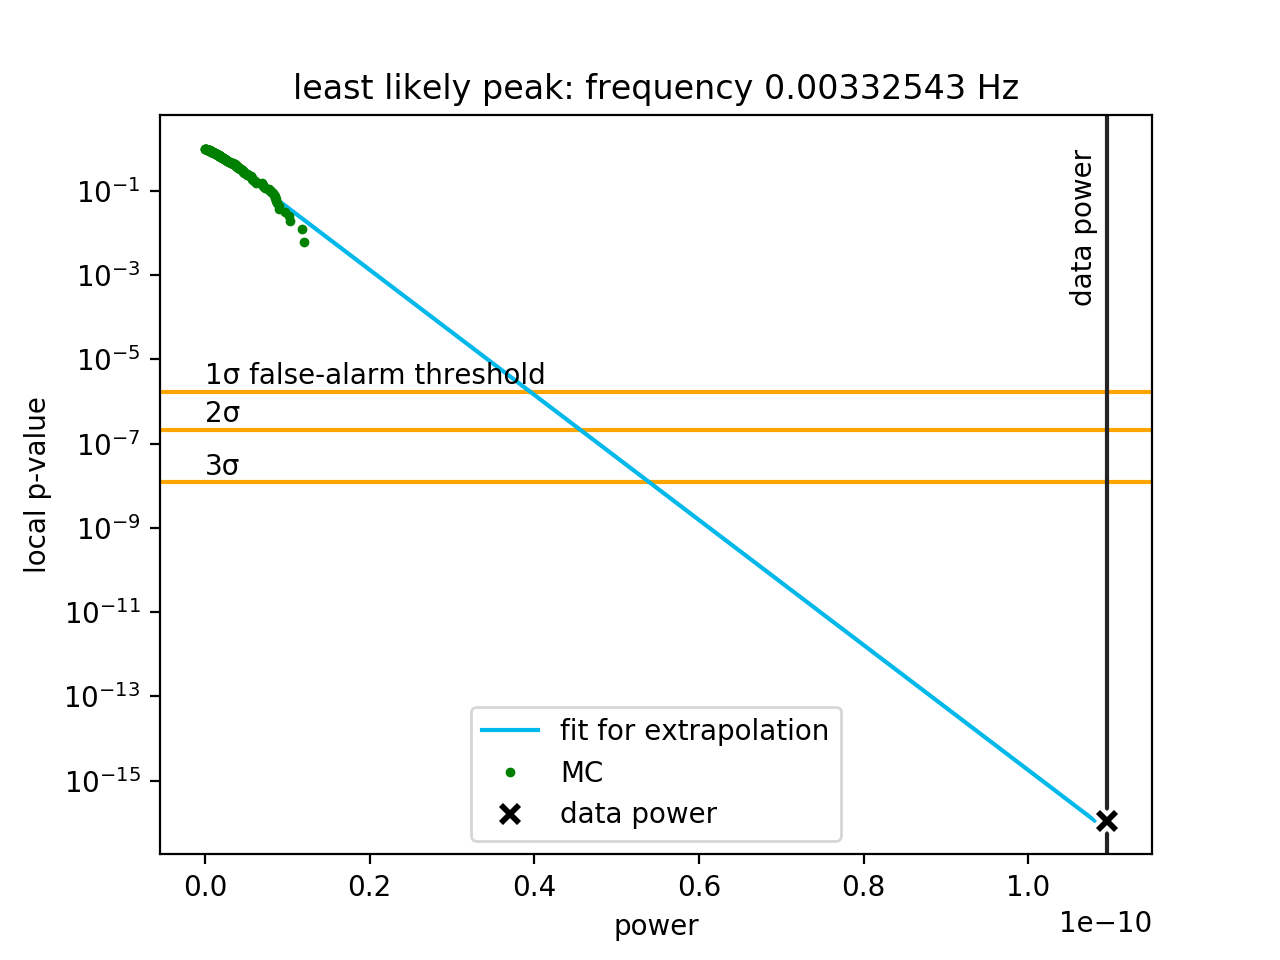
\includegraphics[width=0.9\linewidth]{gfx/axions/P_best_signal_candidate.png}
  \caption{1 - CDF for the parallel data set. This provides the power to local p-value transition, for each frequency separately. The extrapolation based on Eq.\ldots is shown.}
  \label{fig:P_best_signal_candidate}
\end{figure}

Once every MC-generated power estimate has a local p-value associated with it, we find for each generated periodogram the minimal local p-value and treat it as a statistic in itself. We estimate the CDF of the minimal local p-value. The result is plotted in Fig.\,\ref{fig:P_look-elsewhere}. The plot can be understood in the following way: it states how probable it is (y-axis) for a peak of a given local significance (x-axis) to occur anywhere in a periodogram. In other words, the y-axis corresponds to the \emph{global} p-value. The global p-value for an $n\,\sigma$ level is given by:
\begin{equation}
  \mathrm{erfc}\left( \frac{n}{\sqrt{2}} \right)\ ,
\end{equation}
where $\mathrm{erfc}$ is the complementary error function (intuitively understood as ``one minus the integral of the gaussion distribution''). We mark the global p-values corresponding to $1,\ldots,5\sigma$ levels and via the CDF find the corresponding local p-value thresholds.

\begin{figure}
  \centering
  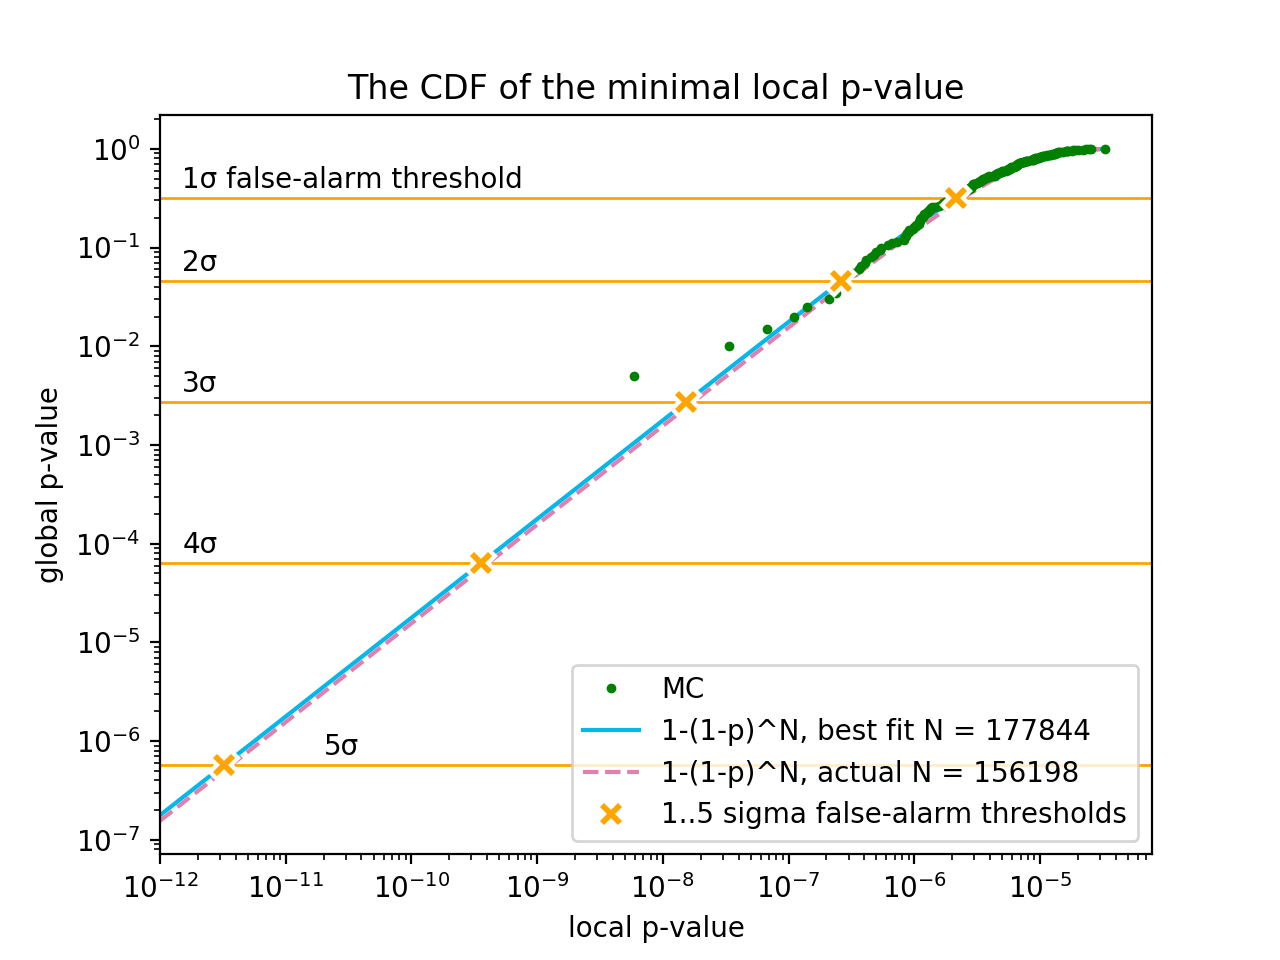
\includegraphics[width=0.9\linewidth]{gfx/axions/P_look-elsewhere.png}
  \caption{Accounting for the look-elsewhere effect for the parallel dataset. It provides the minimal local p-value---global p-value transition. The fit with the model \dots gives the number of frequencies.}
  \label{fig:P_look-elsewhere}
\end{figure}

We see, that the discrete estimate from the MC simulation can only go down to the $2\sigma$ false-alarm threshold. To go lower would require many more MC samples. To observe a single $5\sigma$ event, roughly one-in-a-million, needs typically a million samples. To reduce the computational effort we exploit the fact, that we know the expected functional form of the CDF\@:
\begin{equation}
  F(p) = 1 - (1-p)^N\ ,
\end{equation}
\mnote{Ref.\,for the formula? PDF statistics? Scargle?}
where $N$ is the total number of frequencies. This corresponds to $N$ \emph{independent} statistical tests. We refrain from using for $N$ the actual number of frequencies, \num{156198}, because we cannot guarantee that the power estimates at different frequencies are independent\footnote{They are in a case of periodograms of evenly sampled series}. Instead, we fit $N$ to the observed CDF obtaining \num{177844}. CDFs corresponding to both values of $N$ are depicted in Fig.\,\ref{fig:P_look-elsewhere} and are almost overlapping.

Now for each frequency the local p-values corresponding the the false-alarm thresholds are known. They are depicted in Fig.\,\ref{fig:P_best_signal_candidate}. There, the power CDF (at this frequency) can be used to express the thresholds in power or evaluate the global significance of an arbitrary power. Here, too, the problem is that the discretely estimated CDF does not reach far enough in the tails, and, again, we exploit the functional form to extrapolate the CDF. We expect the power to be exponentially distributed in a no-signal case \cite{Scargle1982}, which corresponds to a straight line on the CDF plot with a logarithmic y-scale.

The thresholds powers are different for each frequency and are depicted in orange in Fig.\,\ref{fig:axions_PSI_detection}. They provide an intuitive interpretation of the plot: the most significant signal candidate is the one piercing furthest into the false-alarm thresholds. Its statistical significance is equal to the last threshold it crossed.



\section{Further discussion}
\mnote{In this paragraph discuss the the distribution of the p-values and plot the filtered p-values.}
\mnote{Now, proceed to discuss the distribution of p-values. Then, proceed to plot the filtered p-values as the function of frequency.}
There are a number of frequencies where statistically significant (put the $\sigma$ level here) excesses are observed in the EB parallel and EB anti-parallel datasets. 
Even though they are not compatible with an axion-induced signal, it is interesting to investigate the possible reason.

In the first step we look at the p-value distribution, shown in black in Fig.\,\ref{fig:axions_P_p-values} (for the EB parallel dataset).
\mnote{Come up with a nice name for the EB parallel and anti-parallel data sets.}
The distribution is flat with narrow peak in the first bin, corresponding to the highest excesses.
This means that there is only a small number (around 300) frequencies, where more power than expected is observed.
\marginpar{A global, like over- or underestimating the error-bars, would cause a tilt in the p-value distribution.}
To identify this group we plot the ratio of the observed to average amplitude (Fig.\,\ref{fig:axions_observed-predicted_power_ratio_filtered}). The lines are low-pass filtered to average the statistical noise out. The excesses occur only for frequencies below \SI{1e-4}{\hertz} and in a narrow region around inverse \SI{300}{\second}. These are the regions where the gradient-drift correction had an effect.

Here tell how it might be due to the imperfect gradient-drift correction. Say, that the narrow region around inverse \SI{300}{\second} is most likely strongly correlated with the low frequencies (essentially peak folding around the Nyquist frequency in the case of evenly sampled data.)


\begin{figure}
  \centering
  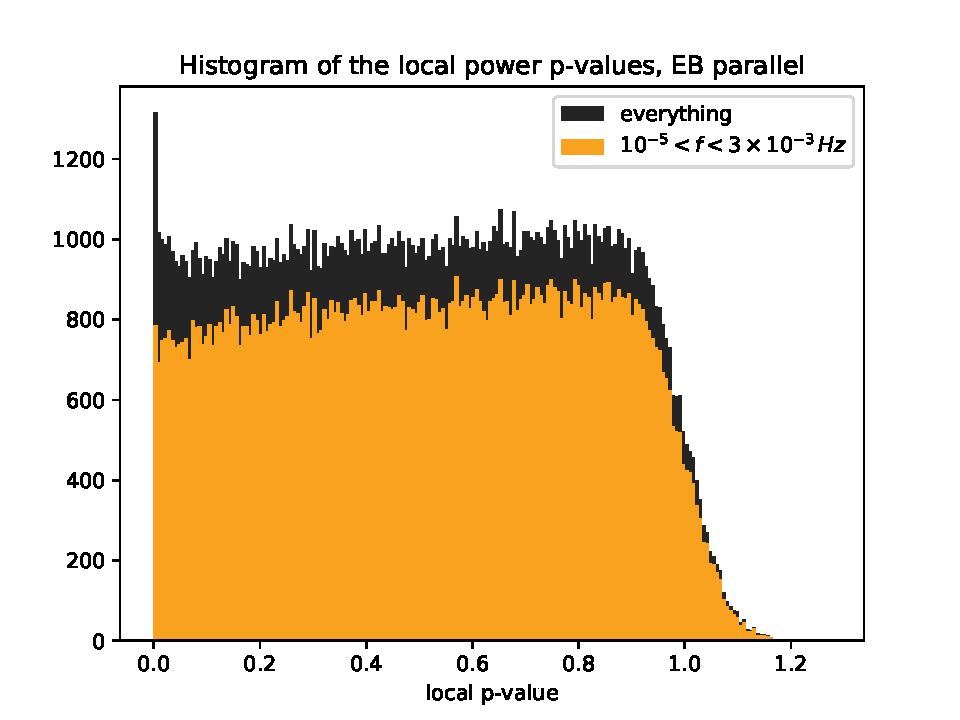
\includegraphics[width=0.9\linewidth]{gfx/axions/P_p-values.pdf}
  \caption{Accounting for the look-elsewhere effect for the parallel dataset. It provides the minimal local p-value -- global p-value transition. The fit with the model \dots gives the number of frequencies. \note{Prepare this histogram in a way, that the curves for all the datasets are shown. Then may need to normalise it.}}
  \label{fig:axions_P_p-values}
\end{figure}

\begin{figure}
  \centering
  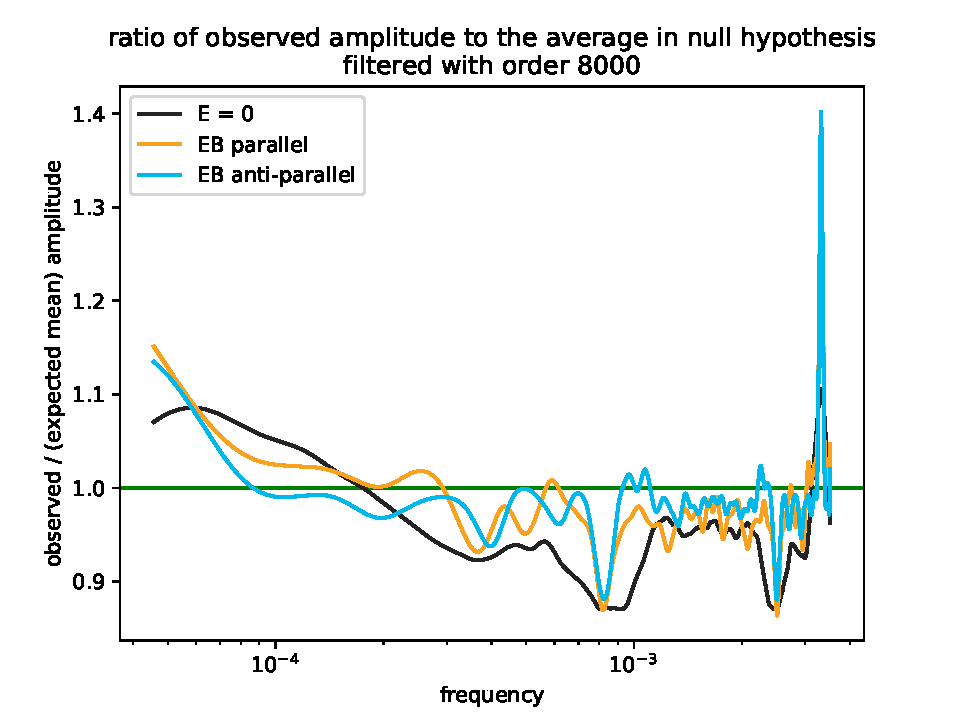
\includegraphics[width=0.9\linewidth]{gfx/axions/observed-predicted_power_ratio_filtered.pdf}
  \caption{Maybe mark the 1/300 seconds. Note, that because of the settling of the filter first $N$ points need to be dropped, so not whole range is plotted.}
  \label{fig:axions_observed-predicted_power_ratio_filtered}
\end{figure}



\section{Axion-Wind analysis}
The analysis described in this chapter so far concerned the scalar coupling of the axions to gluons, which looks like an oscillation in the electric dipole moment of the neutron.
Now we describe how we used the same data set and the same analysis techniques to look for a different coupling --- a vector one of axions to nucleons.

\begin{figure}
  \centering
  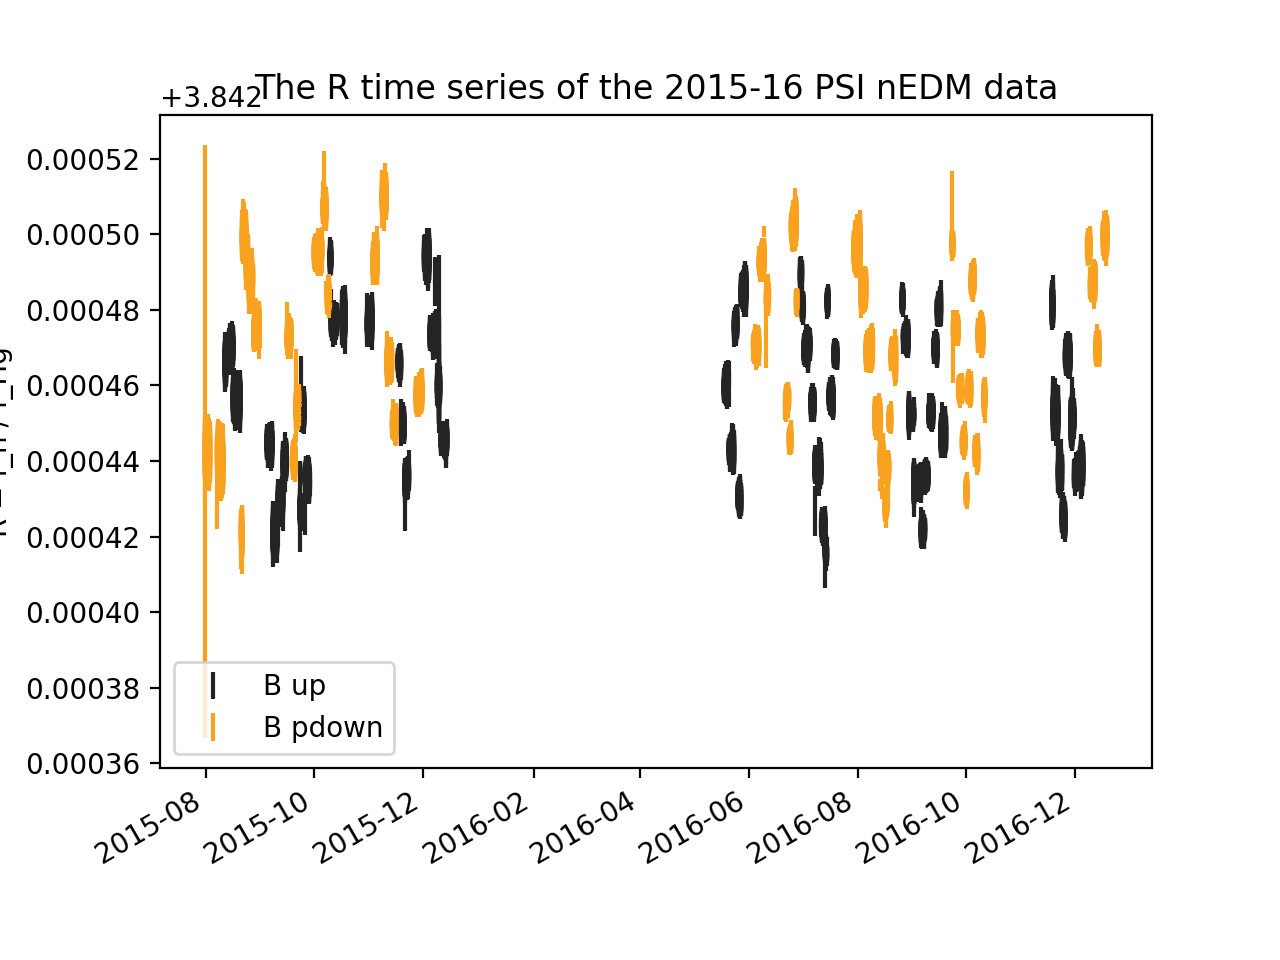
\includegraphics[width=0.9\linewidth]{gfx/axions/winddeltah4mm_time_domain.png}
  \caption{\ldots}
  \label{fig:axions_wind_time_domain}
\end{figure}

This coupling acts like an additional dynamic magnetic field. In this analysis the data are split based on the direction of the holding magnetic field $B_0$, as indicated in Fig.\,\ref{fig:axions_wind_time_domain}. The axion-wind coupling is insensitive to the electric field in the experiment.

The axion-wind coupling \note{ref to equation} is proportional to the projection of experiment's quantisation axis on the momentum of the axions.
Because the latter is due to the Earth traversing the galactic axion field in the Solar System's movement around the Milky Way's centre, the effect is called Axion-Wind. \note{Maybe a ref}
The Earth additionally spins, causing the effect to be modulated with the sidereal frequency $\Omega_\mathrm{sid}$.\footnote{Sidereal frequency is one of the Earth's spinning as seen in the reference of fixed stars.}
The modulation makes a signal in periodogram a triplet, with the central, highest, peak at the frequency of the oscillation of the axion field, and two additional ones, on either side, $\Omega_\mathrm{sid}$ away from the main peak.

Besides splitting the data on the direction of the magnetic field, rather than the relative direction of the magnetic and electric ones, the analysis is performed exactly in the same way as in the case of the search for the scalar axion-gluon coupling. The periodograms for the two datasets are presented in Fig.\,\ref{fig:axions_wind_Bup_detection} (magnetic field pointing upwards, relative to gravity) and Fig.\,\ref{fig:axions_wind_Bdown_detection} (pointing downwards).

\begin{figure}
  \centering
  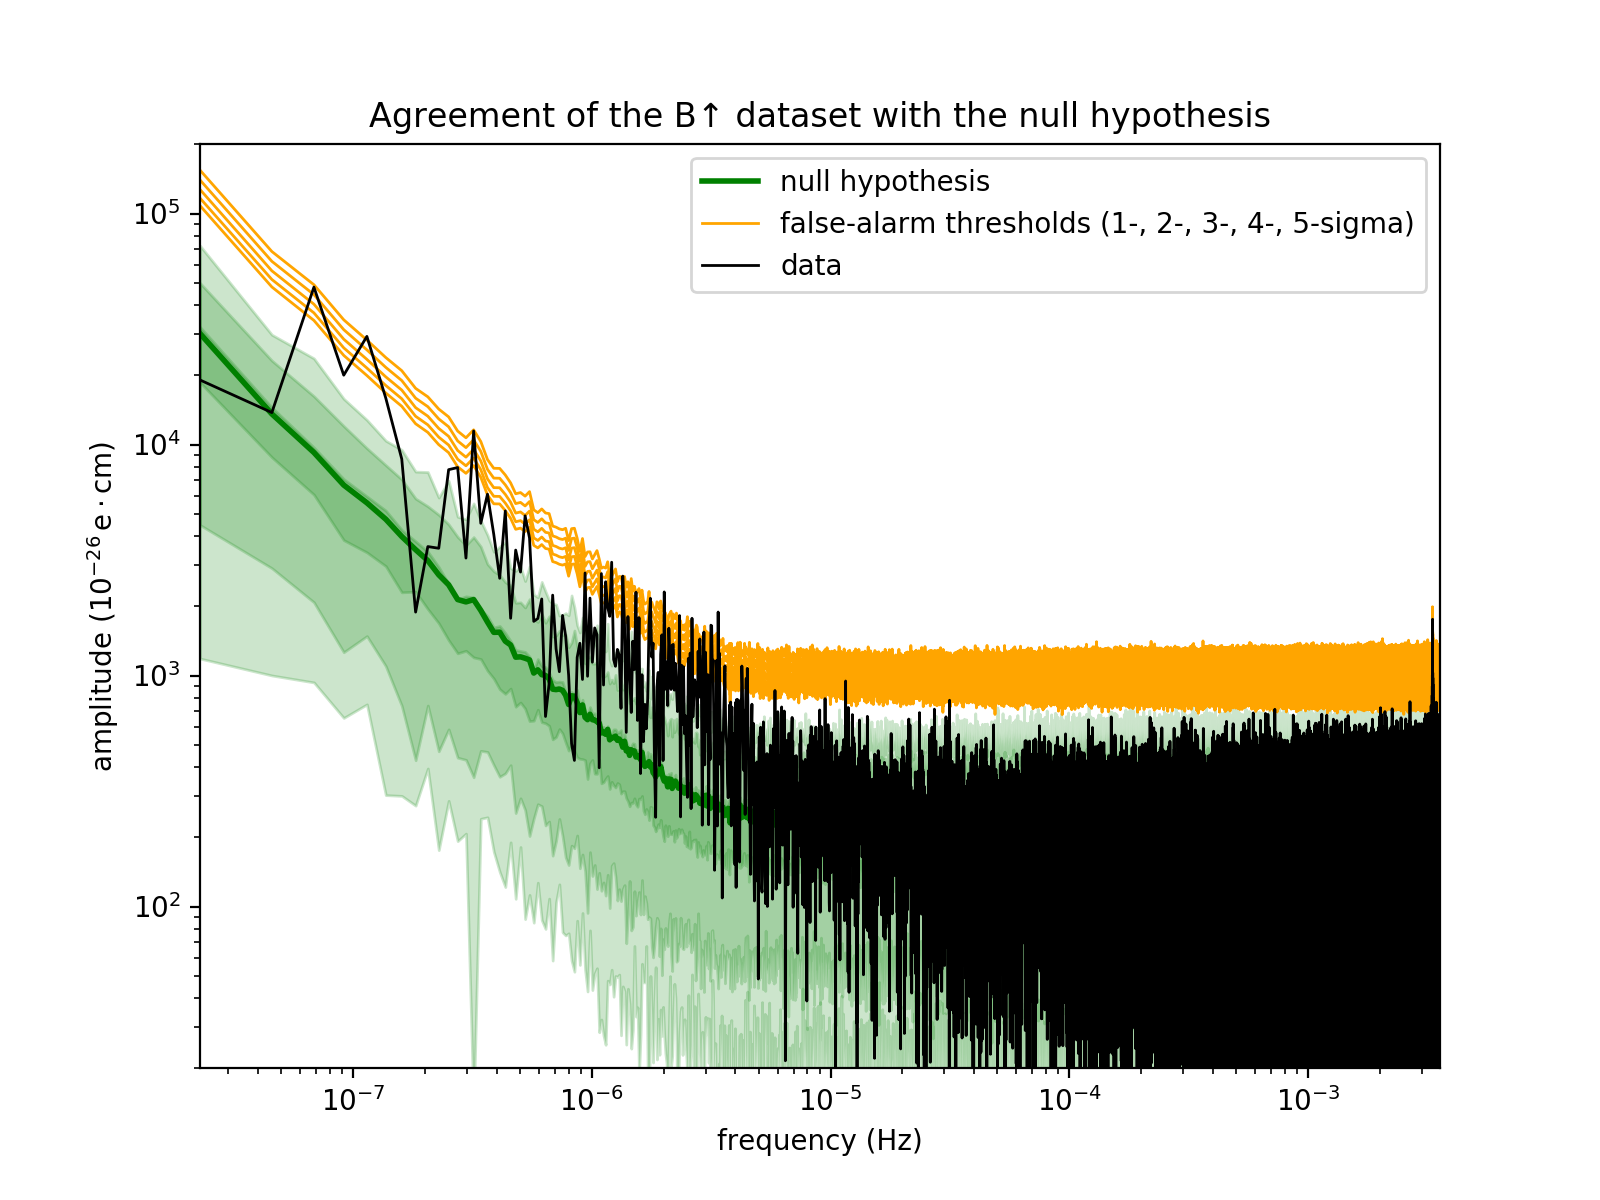
\includegraphics[width=0.9\linewidth]{gfx/axions/winddeltah4mm_Bup_detection.png}
  \caption{Maybe mark the 1/300 seconds. Note, that because of the settling of the filter first $N$ points need to be dropped, so not whole range is plotted.}
  \label{fig:axions_wind_Bup_detection}
\end{figure}

\begin{figure}
  \centering
  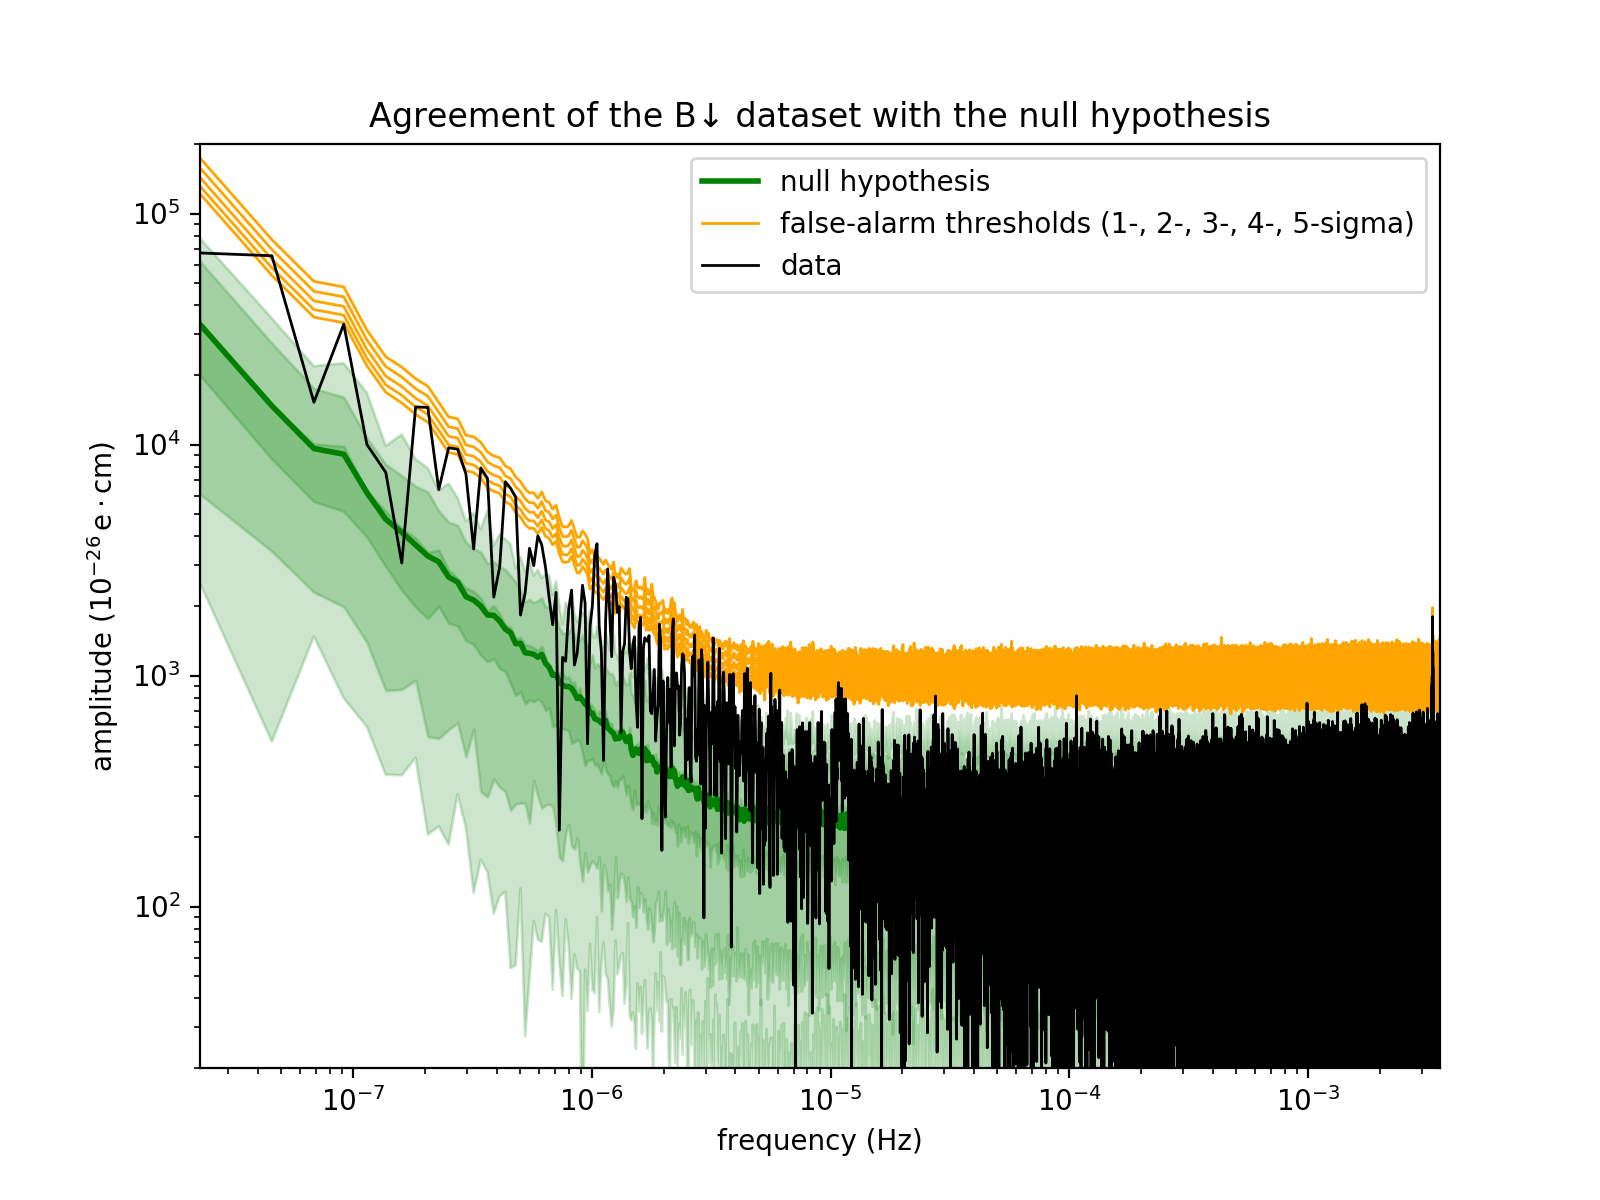
\includegraphics[width=0.9\linewidth]{gfx/axions/winddeltah4mm_Bdown_detection.png}
  \caption{\ldots}
  \label{fig:axions_wind_Bdown_detection}
\end{figure}

We see a lot of excesses (figures, already gradient-drift corrected), but none passes the detection criteria (the phase requirements in particular).

The lack of statistically significant signal compatible with the axion model allowed us to put limits on the axion-nucleon coupling, depicted in Fig.\,\ref{fig:axions_wind_limits}. \note{comment a bit on the other limits in the plot}

\begin{figure}
  \centering
  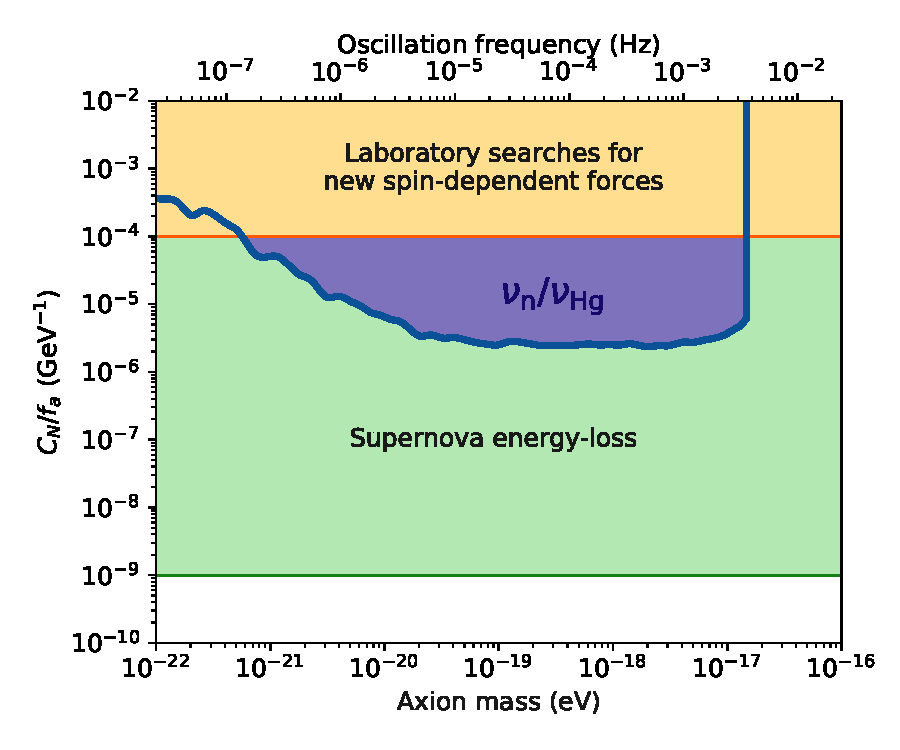
\includegraphics[width=0.9\linewidth]{gfx/axions/psi_ill_axion_wind_limits_v1.pdf}
  \caption{\ldots}
  \label{fig:axions_wind_limits}
\end{figure}



\section{Sidereal frequency}
A note about the signals seen at this particular frequency. Refer to the Lorentz-invariance paper, improve the limit directly? \cite{ALTAREV20112365}



\section{Outlook}
There are three direction in which the nEDM-based axion dark matter search could continue.
To improve sensitivity vertically (be sensitive to more weekly coupled or less abundant axions) the overall sensitivty of the nEDM measurement would need to be improved.
Following the Eq\,\note{ref to the nEDM sensitivity formula}: more neutrons or higher electric field.
\marginpar{In Eq. $\alpha$ is already \ldots, precession time $T$ can only be improved so long --- it is fundamentally limited by the neutron life-time (give the number.)}
The global community already spares no effort to achieve that.
The second way is to improve sensitivity for slower oscillations, or lighter axions, limited by the span of the data set. For this analysis this are the four years of the ILL measurement. Combining the ILL and PSI data into one time series would improve it to \note{number}. It was not done at the time, because the PSI data were still blinded and the run-level analysis was still ongoing.
The third direction is the high-frequency, heavy-axions one. It is limited by the sampling frequency fo the system, the cycle repetition rate. The measurements could be conducted with a shorter cycle time (worsening the sensitivity, as the loss in Eq.\,\note{ref the nEDM sensitivity} is linear, and the gain from the statistics is a square root).
\marginpar{In PSI the cycles are synchronised to the pulses of the kicker magnet, redirecting the proton beam onto the target of the UCN source.}
However, it is hard to imagine going beyond ten-second range. A real improvement in this direction would require changing the principle of the measurement.




\section{Resonant oscillating nEDM search}
Many of the axion searches are resonant based. \note{some references}.
The standard instrument to look for an axion-photon coupling, called a haloscope \note{verity}, consists of ultra-low-noise resonant cavity, where axions can produce photons, detected with an antenna \note{is it an antenna?}.
At any given time the measurement is sensitive only to a narrow band of photon energies (or frequencies), the width given by the finesse \note{verity} of the cavity. To cover a wide range the tuning of the cavity is scanned. In this section an idea of a resonant oscillating nEDM search is pursued.

For polarised neturons in a magnetic field, a transverse oscillating coupling induces a coherent Rabi oscillation between the spin-up and spin-down states.
For example, a Ramsey cycle begins with a $\uppi$/2 flip, induced by an oscillating transverse magnetic field, its frequency tuned to the Larmor one and its length tuned such, that the Rabi oscillation stops when the polarisation is in the transverse plane. Should the nEDM oscillate, an oscillating transverse coupling can be achieved with a static magnetic field \emph{perpendicular} to the holding magnetic field. Then, if the frequency of the nEDM oscillation is tuned to the Larmor one, the neutrons would undergo a Rabi nutation, which could be detected.



First - just scanning.

Broad band possibility? It is like an adiabatic spin-flip, but without the oscillating field. The fact that the spin flip occurs, would indicate a presence of the field.

